% !TEX TS-program = pdflatex
% !TEX encoding = UTF-8 Unicode

% This is a simple template for a LaTeX document using the "article" class.
% See "book", "report", "letter" for other types of document.

\documentclass[11pt]{article} % use larger type; default would be 10pt

\usepackage[utf8]{inputenc} % set input encoding (not needed with XeLaTeX)

%%% Examples of Article customizations
% These packages are optional, depending whether you want the features they provide.
% See the LaTeX Companion or other references for full information.

%%% PAGE DIMENSIONS
\usepackage{geometry} % to change the page dimensions
\geometry{a4paper} % or letterpaper (US) or a5paper or....
\geometry{margin=1in} % for example, change the margins to 2 inches all round
% \geometry{landscape} % set up the page for landscape
%   read geometry.pdf for detailed page layout information

\usepackage{graphicx} % support the \includegraphics command and options

\usepackage[parfill]{parskip} % Activate to begin paragraphs with an empty line rather than an indent
\setlength{\parindent}{1cm}

%%% PACKAGES
\usepackage{booktabs} % for much better looking tables
\usepackage{array} % for better arrays (eg matrices) in maths
\usepackage{paralist} % very flexible & customisable itemizes (eg. enumerate/itemize, etc.)
\usepackage{verbatim} % adds environment for commenting out blocks of text & for better verbatim
\usepackage{subfig} % make it possible to include more than one captioned figure/table in a single float
\usepackage{amssymb} % more 'unusual' symbols not included in standard LaTeX package
\usepackage{enumitem}
\usepackage{amsmath}
\usepackage{color}
\usepackage{xspace}
\usepackage{gensymb}
\usepackage{calligra} 
\DeclareMathAlphabet{\mathcalligra}{T1}{calligra}{m}{n} 
\DeclareFontShape{T1}{calligra}{m}{n}{<->s*[2.2]callig15}{} 

% These packages are all incorporated in the memoir class to one degree or another...

%%% HEADERS & FOOTERS
\usepackage{fancyhdr} % This should be set AFTER setting up the page geometry
\pagestyle{fancy} % options: empty , plain , fancy
\renewcommand{\headrulewidth}{0pt} % customise the layout...
\lhead{}\chead{}\rhead{}
\lfoot{}\cfoot{\thepage}\rfoot{}


%%% SECTION TITLE APPEARANCE
\usepackage{sectsty}
\allsectionsfont{\sffamily\mdseries\upshape} % (See the fntguide.pdf for font help)
% (This matches ConTeXt defaults)

%%% ToC (table of contents) APPEARANCE
\usepackage[nottoc,notlof,notlot]{tocbibind} % Put the bibliography in the ToC
\usepackage[titles,subfigure]{tocloft} % Alter the style of the Table of Contents
\renewcommand{\cftsecfont}{\rmfamily\mdseries\upshape}
\renewcommand{\cftsecpagefont}{\rmfamily\mdseries\upshape} % No bold!

%%%Command Macros
\newcommand{\vf}{\ensuremath{V_{F}}\xspace}
\newcommand{\sr}{\ensuremath{\mathcalligra{r}} \xspace}
%\newcommand{\sr}{\ensuremath{R_{contact}} \xspace}

%%% END Article customizations

\graphicspath{ {./images/} }

\title{The Mimas Leading Edge Anomaly: Thermal conductivity and grain cementation radius estimation}
\author{M.J. Schaible, R.Johnson, L. Zhigilei}
%\date{} % Activate to display a given date or no date (if empty),
         % otherwise the current date is printed 

\begin{document}
\maketitle

\section{'Abstract': Comparison/Summary of thermal conductivity models}

	Here, several thermal conductivity models are discussed and it is seen that there are qualitative similarities shared by all; namely, that the models depend on the thermal conductivity of bulk ice, $k_{ice}$, the porosity, $\phi$, and on geometric factors that depend on the packing of grains. In each of the models, all contributions to thermal conductivity  other than conduction through grains (i.e. radiative, convective, latent heat) are taken to be zero. Conductivity through grains is limited by the contact area between adjacent grains. The models are discussed in more detail in the following and summarized here for ease of comparisson.
	
	\begin{itemize}
	\item Wood (2013)
		\begin{equation}
		k_{eff}  = f_{sc} k_{ice} \frac{\chi + 1 - \phi}{\chi + 1 + \frac{\phi}{2}} \\
		\end{equation}
		
		Where $f_{sc}$ is called the solid continuity factor. It is a measure of the efficiency of contact between adjacent grains and dependent on geometrical packing and contact area, determined by Hertzian analysis and cohesive surface forces (JKR theory), between adjacent grains.
		
		\begin{equation}
		f_{sc} = Y_{sc}N_{c} \left( \frac{N_{c}}{2\sqrt{N_{c}-1}} \frac{R_{con}}{R_{s}} \right)^{Z_{sc}}
		\end{equation}
	
	Here R$_{con}$ is the radius of the contact area, R$_{s}$ is the particle radius, N$_{c}$ is the coordination number, Y$_{sc}$ is determined empirically, Z$_{sc}$ depends on the ratio of solid to void thermal conductivities and, in the case considered here of low temperature and pressure, can be taken to be 1, and the $Y_{sc}$ factor is a fit to experimental data. The coordination number can be calculated exactly for regular packings of monodisperse spheres, with N$_{c}$ = 6 for simple cubic packing, and for small, cohesive, nearly spherical particles Yang et al (2000) gave a functional relationship between coordination number and porosity which closely matches measured and modeled random packings, especially at porosities $\ge$40\%. 
	
	\begin{equation}
	N_{c} = 2.02 \left( \frac{1+87.38(1-\phi)^{4}}{1+25.81(1-\phi)^{4}} \right)
	\end{equation}
		
	Taking $\phi = 0.5$ and assuming $\chi << \phi$ we can simplify this equation to $k_{eff} \approx \frac{2}{5} f_{sc} k_{ice}$. Wood is (apparently) developing an additional model that takes into account the cementation between grains. 
		
%	\item  Piqueuz and Christensen (2009b) \\
%		P and Q did not give explicit equations to calculate the thermal conductivity, but provided several larger plots that traced how the thermal conductivity varied with \% cementation, grain size, gas pressure etc. However, their focus was on ~atm pressure environments, and the model failed for very small grain contact areas (low thermal conductivities), and thus is was determined this model was unfit to explain the regolith at Mimas.

	\item Steiner and K\"{o}mle (1991)
		
		\begin{equation}
		 k_{eff} = \sqrt{1-\phi}\cdot H \cdot k_{ice}(T)
		\end{equation}
		
	Taking $\phi = 0.5$, we can simplify this equation to $ k_{eff} \approx 0.71 H k_{ice}$. The Steiner and K\"omle model uses only the $\sqrt{1-\phi}$ factor to account the the structure of the material. The Hertz factor H is assumed to be similar to the other models. 

	\item Gundlach and Blum (2010)
		
	The Gundlach and Blum model was developed using a mathematical analysis by Chan and Tien (1973) for regularly packed spheres whose contact area is described by Hertzian analysis and where the cohesive forces between spheres are described by JKR theory.
	
		\begin{equation}
		k_{eff} = k_{ice} H \frac{1}{0.531 S(\vf)} \frac{N_{A}}{N_{L}}
		\end{equation}
		
	The factors S$_{vf}$, N$_{A}$, and N$_{L}$ depend on the specific packing arrangement and can be computed explicitly for regular packing arrangements. Note that the porosity of a simple cubic lattice is 47.7\%, close to the 50\% porosity estimated for Mimas. H is the Hertz factor defined as
	
		\begin{equation}
		 H = [\frac{9}{4} \frac{1-\mu^{2}}{E} \pi \gamma r^{2} ]^{1/3}
		\end{equation}
	
	
	\item Sirono and Yamamoto (1997)
		
		\begin{equation}
		k_{eff} = k_{ice} ( \frac{p - p_{c}}{1-p_{c}} )\frac{\pi \sr^{2}}{g r^{2}}
		\end{equation}
		
		Where \sr is the grain contact radius as defined by Hertzian analysis and 'p' is \underline{not} the volume filling factor, but related to it and dependent on the packing. 'p' is the probability that a lattice site is occupied with a regolith grain. The Hertz factor given by Sirono and Yamamoto is slightly different than that of Gundlach and Blum:
		
		\begin{equation}
		H = [ \frac{9 \pi \gamma r^{2} (1-\mu^{2})}{8 E} ]^{1/3}
		\end{equation}
		
	\end{itemize}

\newpage
\section{Introduction}
\label{sec:intro}

	Analysis of Cassini instrument data revealed an anomalous region present on the leading edge of the Saturnian icy moons Mimas and Tethys. The feature was first identified by the VIMS (Visual and Infrared Mapping Spectrometer) instrument as a lens shaped darkening compared to the surrounding regions [Shenketal2011]. It was seen most clearly by taking the ratio of IR/UV light, and the discoloration was centered a 0$\degree$ lat. and 0$\degree$ lon. on the leading edge and extended $\sim \pm30\degree$ to the north and south while spreading over $\>180 \degree$ along the equator. The smaller IR/UV ratio in the anomalous region as compared to surrounding regions was explained as increased scattering at UV wavelengths due to a higher concentration of defects in the icy regolith grains, possibly caused by energetic particle bombardment. Later, using the CIRS (Cassini InfraRed Spectrometer) instrument which measured the thermal IR regime, the emission from the surface was determined during the day and night cycle. Subsequent analysis showed that the temperature variation within a lens shaped region was greater than the surrounding area, indicating a greater thermal conductivity of the material in the lens shaped region, and the spatial extents closely matching the IR/UV discoloration,  [Howettetal2011]. 

	The location of the anomaly was subsequently shown to closely match the expected deposition profile of high energy ($\>$1 MeV) electrons rapidly moving along the magnetic field lines perpendicular to the rotational plane with a high bounce frequency such that they are condenssed out as soon as the magnetic field line crosses the surface. Unlike the thermal plasma, these electrons travel with their net guiding center of motion opposite the rotation direction of the Mimas and Thethys and thereby deposit energy preferentially on the leading edge of these bodies [Paranicasetal2012]. The electons could create scattering centers in the icy regolith which would lead to the observed IR/UV discolorations, and furthermore sintering could lead to increased grain contact and thus explain the anomalous thermal inertia.  The surfaces of the moons are composed almost entirely of crystalline water ice, while essentially free of organic species [Filacchioneetal2010], and the energy deposition due to these electrons was hypothesized to be responsible for an increased sintering volume between the ice grains.

	A good deal of thermal modeling has been done to understand the structure of comets and the thermal inertia of other bodies such as the Moon and Mars. However, the Saturnian moons are composed of water ice as opposed to a rocky regolith and lack the dark organic layer which found on the surface of comets. Also, since the moons lack an atmosphere the thermal conductivity is dominated by intergrain contacts while the thermal conductivity due to gas convection in the regolith is negligible. The purpose of this note is to quantitatively estimate the expected relative contact area or grain sintering radius based on the measured parameters of thermal inertia and grain size. The estimate assumes that both the ice grains and the cementation volume is entirely crystalline, although amorphous ice could be present. The structure of the ice will be discussed in more detail later in this note. 
	
	%REJ - One nice thing would be to correlate defect production--determing the IR/UV ratio to energy deposition--for which there are expressions and then show that that amount of energy deposition is also consistent with your model of the sintering 

\subsection{Thertmal Inertia ($I$) and Skin Depth ($\delta$)}

		Using the measured surface thermal emission excursions, the values for thermal inertia $I=\sqrt(kc\rho)$ were extracted by Howett et al (2011, 2012). Using the values of thermal inertia and assuming a porosity of $\phi = 50\%$, the thermal conductivity and the skin depths $\delta = \frac{I_{out}}{(1-\phi)\rho_{ice} c \sqrt{\omega}}$ inside and outside the anomalies were determined and are given in table 1, where $c$ is specific heat taken as 0.82 MKS, $\rho_{ice}$ is the density of bulk ice (9340 kg/m$^{3}$), and $\omega$ the angular velocity of rotation. The skin depth of calculated assumes that the conductivity is that of porous, crystalline ice regolith. However, the contact area between grains formed by sintering could have different conductivity. 

	\begin{tabular}[c]{ l | l | c | c | c }
	Body & Location & Thermal Inertia & Skin Depth & Thermal Conductivity \\
	& & $\left[ \frac{J}{m^{2} s^{1/2} K} \right]$ & [cm] & $\left[ \frac{J}{m\cdot s\cdot K} \right]$ \\ \hline
	Mimas & Inside anomaly & 66 $\pm$23 & 2.01 $\pm$0.7 & 1.13 $\left(\substack{+0.94 \\ -0.65} \right) \times$ 10$^{-2}$ \\
		& Outside anomaly & $<$16 & $<$ 0.49 & $<$ 6.7 $\times$ 10$^{-4}$) \\ \hline
	Tethys & Inside anomaly & 25 $\pm$3 & 0.76 $\pm$0.09 & 1.63 $(\pm 0.4) \times$ 10$^{-3}$ \\
		& Anomaly boundary & 11 $\pm$1 & 0.34 $\pm$0.03 & 3.16 $(\pm 0.6) \times$ 10$^{-4}$ \\
		& Outside anomaly & 5 $\pm$1 & 0.15 $\pm$0.03 & 6.53 $\left(\substack{+2.9 \\ -2.4} \right) \times$ 10$^{-5}$ \\
	\end{tabular}

	The average path length traveled by $1 - 10 MeV$ electrons impacting on water, calculated with the ESTAR program using the continuous-slowing-down-approximation (CSDA), is $0.4-5.0 g/cm^{2}$, which for $50\%$ porous water ice gives $0.85-10.6 cm$ total path length [NIST, e-star]. \textcolor{red}{Unfortunately, the NIST data does not give a projected range for the electrons (depth of penetration).} The depth of penetration into the material must be less than the total path length, but due to efficient scattering effects from electron-nucleus and electron-electron interactions, the actual electron penetration depth varies. For light materials such as water ice, the maximum depth is expected to be on the order of the CSDA range [Attix, 2008]. The similarity in the penetration depths of the electrons and the skin depth of the thermal anomaly suggest that the electrons could be responsible for the increased thermal conductivity.  
	
	Here we show that a possible explanation for the thermal conductivity differences could be sintering in an intergrain contact region due to energy deposited in electronic excitations of the water molecules either on the surface or in the bulk of the ice grains. The deposited energy can mobilize water molecules, causing them to migrate along the grain surface or desorb from the surface to be redeposited in the intergrain region. This can lead to grain growth and, more importantly, growth in the size of the contact regions between grains and improved thermal contact  across the grain boundaries.
	
	 As discussed below the same energy deposition that mobilizes the water at the grain boundaries can cause defects in the bulk. Whereas sintering increases the effective thermal conductivity, such defects, which we assume to be the principal cause of the increase in the IR/UV ratio, can cause a decrease in thermal conductivity. However, below we will also show that the density of bulk defects produced at a level consistent with the sintering are sufficient to affect the UV scattering but not to significantly affect the thermal conductivity.
	
%\emph{There should be a pressure minimum in the pendular region. Need equation to explain. Another argument in the minimization of surface energy. Need to look more into that too.}
	
\section{Contributions to the effective thermal conductivity of an icy porous regolith}

	In general, the thermal conductivity of a granular, uncemented sample under vacuum can be separated into a conductive which describes heat flow through the bulk, and a radiative term which describes heat flow through the void space [Watson, 1964]. 
	
	\begin{equation} \label{eq:TCbasic}
	k_{eff} = A T^{3} + B
	\end{equation} 
	
	The first term depends on both grain size and porosity and is due to radiation as dicussed further below in \ref{sec:krad}. The second factor was given by Watson (1964) as $B = \frac{3000}{D}\times10^{-5}$ for $D > 2m \mu m$ and is a function of the bulk conductivity, $k_{grain}, and the contact area, $S$, between grains. For porous regoliths typical of airless solar system bodies heat flow is limited by the  amount of intergrain contact.

	A and B can be measured empirically for a given material, or modeled as hard spheres and calculated computationally, though variations in porosity, vacuum conditions and grain size can be difficult to study in the lab and using solid sphere computational models may miss important effects from the regolith microstructure. However, much work has been done to constrain the various parameters that affect the thermal conductivity, and those possibly relevant to Mimas and Tethys will be outlined and their usefulness for describing the effective thermal conductivities reported by Howett et al, (2011, 2012) is discussed below. 

\subsection{Radiative contribution to thermal conductivity}
\label{sec:krad}

	The contribution to thermal conductivity from radiative heat emission from the grain/pore surfaces, the first term in ~\ref{eq:TCbasic}, can be estimated as [Kasparek and Vortmeyer, 1976]

	\begin{equation}
	k_{rad} = 4 \psi D \sigma T^{3}
	\end{equation}
	
	where $D$ is the particle diameter, $T$ it the temperature, $\simga$ is the Stephan Boltzmann constant, and $\psi$ is a heat transport coefficient defined by
	
	\begin{equation}
	\psi = \frac{2F + \epsilon'(1-F)}{2(1-F)-\epsilon'(1-F)}
	\end{equation}

	for which F is a 'radiative constant' equal to $\approx$ 0.08 and $\epsilon'$ is related to the emissivity $\epsilon$ of the material by $\epsilon' = \frac{\epsilon}{\epsilon +0.5(1-\epsilon)}$. Taking $D = 50 \mu m$, and $\epsilon = 1$, then the radiative contribution to the thermal conductivity can be estimated as $k_{rad} \approx 6.3\times10^{-6} \frac{J}{m \cdot s \cdot K}$.
	
	\begin{equation}
	\begin{split}
	\Rightarrow \epsilon' &= 1 \\
	\Rightarrow \psi &= \frac{1+F}{1-F} \approx 1.087 \\
	\Rightarrow k_{rad} &= 4 (1.087)(5\times10^{-5} m)(5.67\times10^{-8} \frac{J}{m^{2} s K^{4}}(80 K)^{3}) \\
	\Rightarrow k_{rad} &= 6.3\times10^{-6} \frac{J}{m \cdot s \cdot K}
	\end{split}
	\end{equation}

	Thus we see that the radiative contribution at appoximate Mimas temperatures can account for only $\approx 1/3000$th of the total thermal conductivity as measured for the anomalous region on Mimas, though it could account for 1/10th of the thermal conductivity outside of the anomalous region on Tethys. Since the radiative contribution is generally $<1\%$  of the total thermal conductivity, it will be neglected in the remainder of our analysis.

\subsection{Latent heat contribution to thermal conductivity}
	The thermal conductivity of the void space depends not only on the radiative heat transfer across the void space, but also convective heat transfer due to gas pressure in the pores and sublimation of $H_{2}O$ into the vacuum. In vacuum the gas pressure is low enough that the the former mechanism can be neglected, and the latter process can be described by the Hertz-Knudsen formula:

	\begin{equation}
	k_{lat} = ( \frac{m}{2 \pi k_{B} T})^{1/2}  (L S) \frac{dP}{dT}
	\end{equation}
	
	where $m$ is the mass of the gas molecule, $k_{B}$ is the Boltzmann constant, $L$ is the latent heat of sublimation per unit mass and $S = \phi d$ is the average pore size dimension where $\phi$ is the porosity and $d$ the average particle diameter. $P$ is the vapor pressure of the gas of interest and is given by the Clausius-Clapeyron equation:
	 
	 \begin{equation}
	 P = ae^{(-b/T)}
	 \end{equation}
	 
	 where $a$ and $b$ are experimentally determined parameters given for water vapor over ice by Fanale et al. (1986) as $a = 3.56 \times 10^{12} N m^{-2}$ and $b = 6141.667 K$. Note that both convective and advective contributions to the heat flux are negligible compared to the latent heat effect at the presures expected for Mimas. Taking the latent heat of sublimation to be $L = 48600 [\frac{J}{mol}]$ and again using a temperature of 80 K, the contribution to thermal conductivity from the latent heat is given as:
	
	\begin{equation}
	\begin{split}
	k_{lat} = [ \frac{18 \frac{g}{mol} \times N_{A}}{2 \pi k_{b} (80K)} ]^{1/2} (48600 \frac{J}{mol} & \times N_{A})(0.9 \cdot 50\times10^{-6} m) [ \frac{(3.56\times 10^{12} \frac{N}{m^{2}})(6141.7 K)}{(80 K)^{2}} exp( \frac{-6141.7}{80} ) ] \\
	\Rightarrow k_{lat} &= 1.15\times10^{-26}\frac{J}{m \cdot s \cdot K}
	\end{split}
	\end{equation}
	
	At 80K, the thermal conductivity due to latent heat of sublimation is completely negligible, and thus the total void thermal conductivity can be taken as due to radiative heat transfer and by extension the void thermal conductivity contributes a negligible amount to the total thermal conductivity of the regolith. 

\subsection{Analytical models of conductive heat transport mechanisms in a porous icy regolith}
	There are several methods in the literature for determining the thermal conductivity of a grainy regolith that take into account grain size, porosity, and a cementation or contact area between adjacent grains. For cold grainy regoliths, the thermal resistance is dominated by the intergrain contact area and increases in the contact lead to increases in the thermal conductivity. In the following we will review several approaches to modeling the thermal conductivity of an icy regolith including cementation between grains.

\subsubsection{From Piqueux and Christensen (2009b): Problem of applicability}

	 Piqueux and Christensen (2009) were primarily concerned with the effect of gas pressure in the voids between grains, but their results also considered low gas conductivities ($<1x10^{-5}$) which approach the thermal conductivity of vacuum. Based on Figure 8 from that paper, the percent volume fraction of cementation is below the lowest value they studied, not including their results for zero cementation. 

	 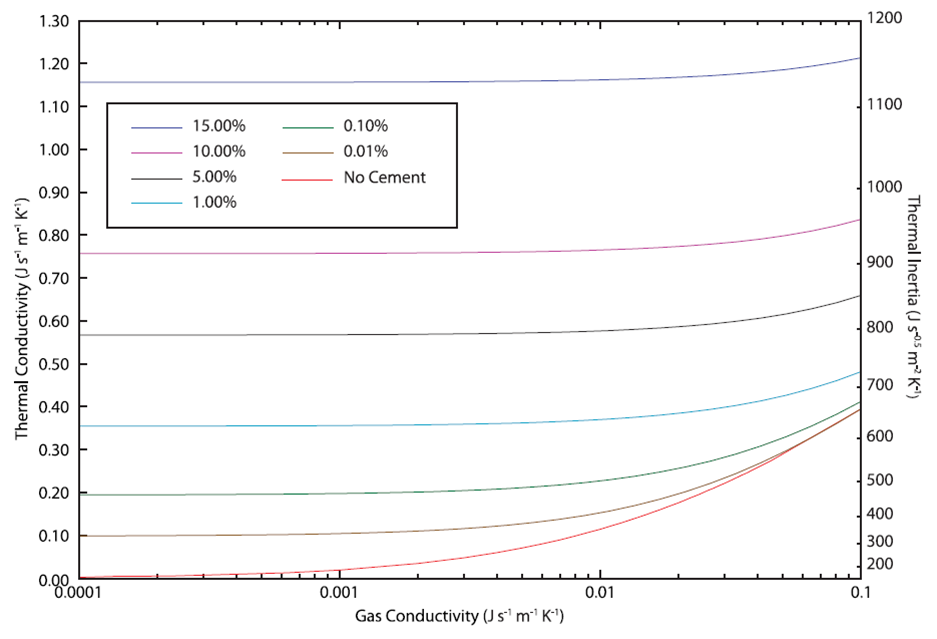
\includegraphics[scale=0.5]{PandQ2009b_CementVolumeFraction.png}

	The image shows that the measured thermal conductivity inside the anomaly ($k_{in} = 0.0113 \: J/(m \cdot s \cdot K)$) falls well below the minimum cement volume fraction used by P and C. However, it can be seen that, for vanishing gas conductivity,  the relationship between the cement volume fraction and thermal conductivity can be approximated by $V_{cem} \varpropto 21\cdot k_{eff}^{3.32}$. Thus, the volume fraction of cement inside and outside the anomaly was estimated as:
	
	\begin{itemize}
	\item $\chi_{in} \approx 7\times10^{-6}\%$
	\item $\chi_{out} \approx 5\times10^{-10}\%$
	\end{itemize}
	
	It should be noted that the grain thermal conductivity used was only 0.937 MKS, while the cement thermal conductivity used in the graph above was 6 MKS. However, the effects of varying these parameters were explored in several other plots in their paper, and it can be seen that for very low cement volume fractions the cement thermal conductivity does not effect the effective thermal conductivity and for all cement thermal conductivities evaluated the effective thermal conductivity approaches a single value dependent on grain size and pore gas pressure. Though the effect of varying the grain thermal conductivity was not discussed in the paper, it can be assumed to be negligible because the effective thermal conductivity is controlled by the cementation between grains. Furthermore, it is stated in the paper that '\emph{for extremely small volumes of bonds ($< 0.01\%-0.001\%$) the bulk thermal conductivity remains mostly unchanged and is a function of ... temperature and grain size}'. We see that the determined values for cement volume fraction are well below these limits, and thus the model of P and Q is not adequate to estimate the cementation between grains. 

\subsubsection{Wood (2011, 2013): Empirical fitting and packing dependences}
	 Wood (2011, 2013) modeled heat transfer through a grainy porous regolith as being due to conduction through grains and gas filled pores and radiation from grain surfaces across pores, with each thermal path acting in parallel so that $k_{eff} = k_{c} + k_{r}$, where $k_{c}$ and $k_{r}$ represent the conductive and radiative components of the effective thermal conductivity, respectively. Taking $k_{r}$ to be negligible, as discussed above, we are left with:
	
	\begin{equation}
	k_{c} = k_{c,min} +f_{sc}(k_{c,max}-k_{c,min})
	\end{equation}
	
	which represents both the gas and solid conduction paths. Here, $k_{c,min}$ is the minimum conductive thermal conductivity which, for the low pressure environments of Mimas and Tethys, can be taken to be zero, and $k_{c,max}$ is determined by the thermal conductivity of the grain material,$ k_{s}$, the porosity $\phi$, the volume percent and thermal conductivity of cementation region, $\chi$ and $k_{cem}$ respectively, and  $f_{sc}$ is the fractional continuity of the solid phase and is discussed further below. Taking the Wood model at low pressures, we find
	
	\begin{equation}
	\begin{gathered}
	k_{c,min} \rightarrow 0 \\
	k_{c,max} = \frac{k_{cem}\chi + k_{s}\nu_{s}\frac{3k_{cem}}{2k_{cem}+k_{s}}}{\chi +\nu_{s}\frac{3k_{cem}}{2k_{cem}+k_{s}}+\phi\frac{3k_{cem}}{2k_{cem}}} \\
	\\
	\text{where  } \phi = (1-\nu_{s})\\ 
	\end{gathered}
	\end{equation}

	Assuming that both the cementation region and the bulk grains are crystalline ice, $k_{s} = k_{cem} = k{ice}$, this equation can be simplified and we can write the effective thermal conductivity as:
	
	\begin{equation}
	\begin{gathered}
	k_{c,max} = k_{ice} \frac{\chi + 1 - \phi}{\chi + 1 + \frac{\phi}{2}} \\
	\Rightarrow k_{eff} = f_{sc} k_{c,max} = f_{sc} k_{ice} \frac{\chi + 1 - \phi}{\chi + 1 + \frac{\phi}{2}} \\
	\\
	\text{assuming   } \chi << \phi  \Rightarrow k_{eff}=2 f_{sc} k_{ice} \frac{1-\phi}{2+\phi}
	\end{gathered}
	\end{equation}
	
	The $f_{sc}$ factor represents the effect of interparticle contact and/or cementation and is a measure of the efficiency of contact between adjacent grains. The factor contains both geometrical and contact area considerations and, for uncemented soils, is given in terms of the size and number of contacts per particle, where contact size is determined by Hertzian analysis and cohesive surface forces (JKR theory).
	
	\begin{equation}
	f_{sc} = Y_{sc}N_{c} \left( \frac{N_{c}}{2\sqrt{N_{c}-1}} \frac{R_{con}}{R_{s}} \right)^{Z_{sc}}
	\end{equation}
	
	where R$_{con}$ is the radius of the contact area, R$_{s}$ is the particle radius, N$_{c}$ is the coordination number, Y$_{sc}$ is determined empirically, and Z$_{sc}$ depends on the ratio of solid to void thermal conductivities and, in the case considered here of low temperature and pressure, can be taken to be 1. The coordination number can be calculated exactly for regular packings of monodisperse spheres, with N$_{c}$ = 6 for simple cubic packing which has a porosith of 47.64\%, similar to the porosity used here. For polydisperse mixtures of randomly packed particles the coordination number cannot be known exactly, but for small, cohesive, nearly spherical particles Yang et al (2000) gave a functional relationship between coordination number and porosity which closely matches measured and modeled random packings, especially at porosities $\ge$50\%. 
	
	\begin{equation}
	N_{c} = 2.02 \left( \frac{1+87.38(1-\phi)^{4}}{1+25.81(1-\phi)^{4}} \right)
	\end{equation}
	
	Using a porosity of 50\%, we find the coordination number is N$_{c}$ = 4.99. However, for non-spherical particles the shape and orientation of a particle can have an effect on the number of contacts and thus the porosity is less strongly coupled to the coordination number. The equilibrium contact radius between two elastic spheres of the same radius R$_{s}$ under a mechanical load can be calculated from JKR theory (Johnson et al., 1991) and is discussed in more detail for non-spherical particles by Wood (2013). The remaining factor for the to be determined, Y$_{sc}$, is determined by comparrison with laboratory measurements. The analysis performmed by Wood (2013) for a variety of glass bead samples of various size distributions revealed that Y$_{sc}$ = 0.09 gave the best overall fit to the data with a mean standard deviation of 13.6\%. Using these values and assuming a mean particle size of 50$\mu$m, we can determine the solid continuity factor and the contact radius. These values are given in table 2. 
	
\subsection{Steiner and K\"{o}mle (1991): Determination of grain sinter radius by Hertz factor analysis}

	A third method of determining the effective thermal conductivity of a porous water ice regolith at low pressure (high Knudsen numbers) was outlined in Steiner and K\"{o}mle (1991) who used expressions given in Tsostas and Martin (1987) to derive:

	\begin{equation}
	k_{eff} = (1-\sqrt{1-\phi})\phi \cdot k_{void} + \sqrt{1-\phi}[H k_{ice}+(1-\phi)\frac{B+1}{B}\frac{k_{ice}k_{void}}{k_{ice}+k_{void}}]
	\end{equation}
	
	where $\phi$ is the regolith porosity, $k_{void}$ is the thermal condictivity across the void region due to a combination of radiative heat transfer and the latent heat of sublimation, $k_{ice}$ is the thermal conductivity of bulk ice, $H$ is the 'Hertz-factor' used to describe the radius of the intergrain contact area, and B is a deformation factor related to porosity by:
	
	\begin{equation}
	B = 1.25 ( \frac{1-\phi}{\phi} )^{10/9}
	\end{equation}
	
%	Using the greater value of $k_{void} = 6.3\times10^{-6} \frac{J}{m \cdot s \cdot K}$ from the analysis above and a thermal conductivity for ice at 80 K of $k_{ice} = 567/T = 7.09 \frac{J}{m \cdot s \cdot K}$, we can analyze the effective thermal conductivity to obtain a comparison of the Hertz factor inside and outside the thermal anomally feature.
	
%	Noting that for a porosity of $\phi = 0.5$, the deformation factor $B = 1.25$, and thus the effective thermal conductivity can be reduced to:

	Taking the thermal conductivity of the void region to be negligible as discussed above, we can simplify the effective thermal conductivity to depend only on the Hertz factor and the porosity of the regolith.
	
	\begin{equation}
%	k_{eff} = (1-\sqrt{1-0.5})(0.5)(6.3\times10^{-6}) + &\sqrt{1-0.5} [ H \cdot 7.09+(1-0.5)\frac{1.25+1}{1.25}\frac{(7.09)(6.3\times10^{-6})}{(7.09+6.3\times10^{-6})} ] \\
%	\Rightarrow k_{eff} &= ( 4.93\times 10^{-6} + 2.24\cdot H )  \frac{J}{m \cdot s \cdot K} \\
	\Rightarrow k_{eff} \approx \sqrt{1-\phi}\cdot H \cdot k_{ice}(T)
	\end{equation}
	
	Using the effective thermal conductivities obtained above for a 50\% porous regolith both inside and outside the anomalies and taking the thermal conductivity of water ice at 80Kto be $k_{ice} = 567/T = 7.09 MKS$ [Kossacki et al., (1994)], we can solve for the Hertz-factor. Here it is worthwhile to note that Hertz-factors used previously in the literature to describe a porous icy cometary nucleus are on the order of  $H  \approx (1 - 4) \times10^{-3}$ [SteinerKomle1991], which compares favorably with the values obtained for the Mimas regolith. 
	
\subsection{Sirono and Yamamoto (1997):}

	Using effective-medium theory, the effective thermal conductivity for a random network of spherical grains arranged on a regular lattice can be determined by integrating the propability distribution of $k$ multiplied by the 1-D heat flux to obtain the effective heat flux, which then yields(Eq. 8 of Sirono and Yamamoto):
	
	 \begin{equation}
	 \frac{k_{eff} - k_{ice}}{k_{ice} +(1/p_{c}-1)k_{eff}}p + \frac{k_{eff}-k_{void}}{k_{void}+(1/p_{c}-1)k_{eff}}(1-p)=0
	 \end{equation}

	 where the probability of a lattice site being occupied or packing fraction is $p$, $p_{c}$  is the percolation thereshold which defines the minimum packing fraction for a continuous thermal path to exist across the material, and $k_{eff}$, $k_{ice}$, and $k_{void}$ are the effective, bulk ice, and void space thermal conductivities respectively. If we take $k_{void} \approx 0$, this equation reduces to:
	 
	 \begin{equation}
	 k_{eff} = k_{ice} \frac{p - p_{c}}{1 - p_{c}}
	 \end{equation}
	 
	 However, this expression does not account for the constuction of heat flow due to reduced area at the grain contacts, and this effect can be taken into account by multiplying by a factor that takes into account the contact area, packing structure, and grain size. The contact area in turn is determined Hertzian analysis
	 
	\begin{equation}
	\begin{split}
	k_{eff} &= k_{ice} ( \frac{p - p_{c}}{1-p_{c}} )\frac{\pi \sr^{2}}{g r^{2}} =  k_{ice} ( \frac{p - p_{c}}{1-p_{c}} )\frac{\pi}{g r^{2}} H^{2} \\
		 &= k_{ice} ( \frac{p - p_{c}}{1-p_{c}} )\frac{\pi}{g r^{2}}[ \frac{9 \pi \gamma r^{2} (1-\mu^{2})}{8 E} ]^{2/3}
	\end{split}
	\end{equation}

\subsubsection{What is the Hertz-factor really?}

	The Hertz-factor is a parameter that describes the amount of deformation between elastic spheres in contact and give the radius of the intergranular contact area. A larger Hertz-factor corresponds to greater interparticle contact, thereby allowing a greater heat flux and a higher thermal conductivity. Thus, for otherwise identical regoliths, the Hertz factor is a parameter that can be used to describe the relative amount of intergranular contact (cementation?). In modeling of thermal conductivity of grainy, porous materials, a common approximate technique is to consider a mono- or polydisperse 'bed' of elastic spheres. The requirement for the spheres to be elastic and not a perfect hard sphere stems from physical considerations, since the contact point of hard spheres is infinitesimal, through which no heat can flow. Therefore, the spheres must deform slightly at the contact point so there is some finite area across which heat can flow. At the atomic scale, the heat transfer through disimilar spheres with no adhesive bonding is due predominantly to the van der Waals intereactions which mediate the phonon transfer, while for cemented grains where there is adhesive material connecting the grains which tranfer heat directly through lattice vibrations. 
	Experimentally, the thermal conductivity is seen to depend exponentially on the volume filling factor $\vf = 1- \phi$, determined experimentally by taking the mass of a given volume of grainy material and comparing to the volume of an equivalent mass of solid material, as [Krause et al, 2011 (via Gundlach and Blum (2012))],:
	
	\begin{equation}
	k(\vf) = c_{1} exp [c_{2} \vf]
	\end{equation}

	where $c_{1}$ and $c_{2}$ are derived by fitting the measured data.
	
	Theoretically, the thermal conductivity of elastic spheres can be explained using the Hertzian theory of contact [Hertz, 1881] to describe the deformation of the interface between spheres. For packed spheres under vacuum ($k_{cond} = 0$), the heat conductivity can be calculated by [ChanTien1973]:
	
	\begin{equation}
	k_{eff}(r, T, \vf) = k_{ice}\cdot \sr \cdot \xi(r, \vf)= k_{ice}(T) [\frac{3}{4} \frac{1 - \mu^{2}}{E(T)} F(r) r]^{1/3} \xi(r, \vf)
	\end{equation}
	
	 where $r$ is the particle radius, $k_{ice}$ is the thermal conductivity of bulk (solid) ice, $\sr$ is the radius of the contact area between touching spheres as described by the Hertz relation, $\mu$ and $E(T)$ are Poisson's ratio and Young's modulus of the material, respectively, and $F(r)$ is an externally applied force which acts on the spheres and determines the contact area between adjacent particles. The packing structure of the material and the number of interparticle contacts is taken into account by $\xi(r, \vf)$ where:
	
	\begin{equation}
	\xi(r, \vf) = \frac{1}{0.531 S(\vf)} \frac{N_{A}(r)}{N_{L}(r)}
	\end{equation}
	 
	 Here, $s(\vf)$ is a 'model parameter' that depends on the packing structure, and $N_{A}(r)$ and $N_{L}(r)$ are the number of particles per unit area and unit length respectivenly.  When no external force is applied, the weight of the particles can be used to determines the force and thus the contact area, but van der Waals bonding can provide orders of magnitude greater adhesive forces and it can be calculated by the JKR theory [Johnson et al (1971)] as:
	 
	 \begin{equation}
	 F_{vdW}(r, T) = 3 \pi \gamma(T) r
	 \end{equation} 
	 
	 where $\gamma(T)$ is the specific surface energy of the material and a measure of the adhesive bonding strength between grain surfaces. It should be noted here that this expression may differ substantially for sintered grains where the boundary may have some degree of crystalline bonding. Substituting the above expression into the conductivity equation, we can define the Hertz-factor as the ratio of the effective (regolith) thermal conductivity and the bulk conductivity:
	 
	 \begin{equation}
	 \label{eq:hertz}
	 H(r, T, \vf) = \frac{k_{eff}(r, T, \vf)}{k_{ice}(T)} = [\frac{9}{4} \frac{1-\mu^{2}}{E(T)} \pi \gamma(T) r^{2} ]^{1/3} \xi(r, \vf)
	 \end{equation}
	 
	 This equation can be modified to describe a porous regolith layer composed not simply of spherical grains, but of grain aggregates which themsleves are composed of ice grains and which have their own unique materials parameters such as volume filling factor, Poisson's ratio, Young's modulus, and specific surface energy. Taking the volume filling factor of the layer to be the product of the volume filling factors of the aggregates themselves (\vf$_{agg}$) and the volume filling factor of the aggregate structure \vf$_{struc}$), i.e. ($V_{F, layer} = V_{F, agg} V_{F, struc}$, we can write the effective thermal conductivity of the layer as:
	 
	 \begin{equation}
	 \begin{split}
	 k_{layer}(r_{0}, R, T, V_{F, struc}, V_{F, agg}) = \\
	 k_{agg}(r_{0}, T, V_{F, agg}) [\frac{9}{4} \frac{1 - \mu_{agg}^{2}}{E_{agg}(T)}  \pi \gamma_{agg}(T) r^{2}]^{1/3} \xi(R, V_{F, struc})
	 \end{split}
	 \end{equation}
	 
	 where $R$, $E_{agg}$, and $\mu_{agg}$ are the radius, Young's modulus, and Poisson's ratio of the aggregates, respectively. Taking $r_{0}$ to be the grain radius (the size of the grains that make up the aggregate), the specific surface energy of the aggregates can be calculated by:
	 
	 \begin{equation}
	 \gamma_{agg}(T) = V_{F, agg} \gamma_{ice}^{5/3}(T)[\frac{9 \pi (1-\mu_{agg}^{2})}{r_{0} E_{ice}(T)}]^(2/3)
	 \end{equation}
	 
	 The thermal conductivity of the aggregates can be calculated as before:
	 
	 \begin{equation}
	 k_{eff}(r_{0}, T, V_{F, agg} = k_{ice}(T) [\frac{9 (1-\mu_{ice}^{2})}{4 E_{ice}(T)}\pi \gamma_{ice}(T) r_{0}^{2} ]^{1/3}\xi(r_{0}, V_{F, agg})
	 \end{equation}
	 
	\emph{ In this expression, the unknown parameters are the volume filling factors, assuming that materials parameters can be found for both the bulk material and the aggregates.}
	
\section{Estimaters based on the models above}
	
\subsection{Grain size comparisson via. Hertz-factor analysis}
	
	If we compare the Hertz-factor as defined by the ratio of the effective and bulk thermal conductivities ~\eqref{eq:hertz}, assuming that the materials parameters ($\mu, E, \gamma$) as well as the packing structure are the same inside and outside the anomaly, the ratio of the grain size inside and outside the anomaly can be determined as:
	
	\begin{equation}
	\begin{split}
	\frac{H_{in}}{H_{out}} &= \frac{k_{in}}{k_{out}} = \frac{r_{in}^{2/3} \xi(r_{in}, \vf)}{r_{out}^{2/3} \xi(r_{out}, \vf)} \\
	\Rightarrow \frac{H_{in}}{H_{out}} &= \frac{r_{in}^{2/3} \frac{N_{A}(r_{in})}{N_{L}(r_{in})}}{r_{out}^{2/3} \frac{N_{A}(r_{out})}{N_{L}(r_{out})}} \\
	& \text{where }\: N_{A}\varpropto \frac{1}{r^{2}} \: \text{and} \: N_{L}\varpropto \frac{1}{r} \\
	\Rightarrow \frac{r_{in}}{r_{out}} &= (\frac{H_{out}}{H_{in}})^{3}
	\end{split}
	\end{equation}
	
	Based on the Hertz-factor analysis, it is seen that the thermal conductivity $k_{cond} \varpropto \frac{1}{r^{1/3}}$, while the thermal conductivity due to radiative heat transfer $k_{rad} \varpropto r$. Therefore, at high temperatures the radiative term will dominate and the thermal conductivity will increase. However, at lower temperatures the radiative contribution is negligible and the thermal conductivity will increase with decreasing particle size, possible due to the increased number of interparticle contacts. 
	
	\begin{equation}
	 \frac{r_{in}}{r_{out}} = (\frac{H_{out}}{H_{in}})^{3} = \fbox{0.00013}
	 \end{equation}

	This comparison estimates that the particle size within the anomaly is ~4 orders of magnitude smaller than the particle size within the anomaly, while comparisons of the measured grain size yield at most a factor of eight (8) difference. Therefore, we can conclude that the variation in thermal conductivity is not due to grain size differences. 
	
\subsection{Using the Hertz-factor to compare cementation radius}

	\hspace{-2 cm}{
	\begin{tabular}[ l ]{ l | l | c | c | c | c | c }
	\multicolumn{2}{c | }{Authors} & Howett (2011, 2012) & \multicolumn{2}{ | c |}{Wood (2013)} & S\&K (1991) & S\&Y (1997) \\ \hline
	& Location & $k_{eff} \left[ \frac{J}{m\cdot s\cdot K} \right]$ & $f_{sc}$ & $R_{con} [\mu m]$ & H [cm$^{-1/3}$] & S [$\mu m^{2}$]\\  \hline
	Mimas & Inside anomaly & $1.13 \times 10^{-2}$ & $3.98 \times 10^{-3}$ & 0.354 & $2.25 \times10^{-3}$ & 17.1 \\
		& Outside anomaly & $< 6.7 \times 10^{-4}$ &  $2.36 \times 10^{-4}$ & .021 & $1.3 \times10^{-4}$ & 1.00 \\ \hline
	Tethys & Inside anomaly & $1.63 \times 10^{-3}$ &  $5.75 \times 10^{-4}$ & 0.051 & 3.25 $\times10^{-4}$ & 2.47 \\
		& Anomaly boundary &  $3.16 \times 10^{-4}$ &  $1.11 \times 10^{-4}$ & 0.028 & 6.30 $\times10^{-5}$ & 0.48 \\
		& Outside anomaly & $6.53 \times 10^{-5}$ &  $2.30 \times 10^{-5}$ & 0.006 & 1.30 $\times10^{-5}$ & 0.01 \\
	\end{tabular} }

	For all analyses, we see that the contact area inside the anomalous region is greater than without, which is in agreement with the increased thermal conductivity for all other factors being constant. 

\subsubsection{Wood 2013}

	Taking the ratio of the contact radius values obtained from the Wood analysis, we find $\frac{R_{cont,in}}{R_{cont,out}} = 16.9$ for Mimas, while for Tethys we find $\frac{R_{cont,in}}{R_{cont,out}} = 25.0$. Interestingly, if we take the square root of these values, we find they match closely with the values obtained below. I am not sure why this is, but I suspect it has to do with my interpretation of the Wood analysis in that the contact radius perhaps represents an area instead of a radius. Not sure...

\subsubsection{Kossacki et al, 1994}

	The following equation is given in Kossacki et al (1994) without proof, where $\sr_{n}$ is the cementation (pendular ring) neck radius, and $H_{0}$ is the initial Hertz factor. 
	
	\begin{equation}
	H = H_{0} (\frac{\sr_{n}}{\sr_{n,0}})^{2} \\
	\end{equation}
	
	If we take the 'initial' value to represent the regolith outside of the anomalous region, we have:
	
	\begin{equation}
	\Rightarrow \frac{\sr_{n, in}}{\sr_{n, out}} = (\frac{H_{n, in}}{H_{n, out}})^{1/2}
	\end{equation}
	
	Using this equaion, we find for$\frac{\sr_{n, in}}{\sr_{n, out}} = 4.17$ Mimas and $5$ for Tethys.
	
\subsubsection{Sirono and Yamamoto, 1997}

	The analysis of Sirono and Yamamoto discusses the contact area explicitly. Assuming a simple cubic packing structure of the grains, the give the relation between porosity and the packing fraction as 
	
	\begin{equation}
	\begin{gathered}
	p = [ \frac{4}{3} \pi ( \frac{1}{2})^{3} ]^{-1} (1 - \phi) \\
	\Rightarrow \text{for } \phi = 0.5 \text{, } p = 0.955
	\end{gathered}
	\end{equation}
	
	and the critical packing fraction as $p_{c} = 1/3$ and $g = 4$. 
	
	Calculating the contact areas, we find:
	
	\begin{equation}
	\begin{gathered}
	S_{in} = \frac{k_{eff, in}}{k_{ice}} \frac{1-p_{c}}{p - p_{c}}\cdot g r_{grain}^{2} \\
	= \frac{0.00113}{7.09} \frac{1-1/3}{0.955-1/3} \cdot (4)(50 \mu m)^2 \\
	\Rightarrow S_{in} = 1.71\times 10^{-11} m^{2} \\
	\text{and } \Rightarrow S_{out} = 1.00\times 10^{-12} m^{2}
	\end{gathered}
	\end{equation}
	
	Of course, since $S = \pi \sr^{2}$, we can calculate the ratio of the contact radius inside and outside the anomaly and find $\frac{\sr_{in}}{\sr_{out}} = ( \frac{S_{in}}{S_{out}} )^{1/2} = 4.14$ for Mimas and $5.0$ for Tethys which is in very close argreement with the value obtained from the analysis of Kossacki et al. 
	
	It is left to determine the growth mechanism of contact area in order to determine if electron impact heating can explain the increased cementation at the grain interface.  
	
\section{Appendix 1: Calculations}

\begin{itemize} 
\item Skin Depth (calculated for Mimas - outside anomaly)
\begin{equation}
\begin{split}
\delta_{out} &= \frac{I_{out}}{\rho_{regolith} c \sqrt{\omega}}  \\
&= \frac{I_{out}}{(1-\phi)\rho_ {ice} c \sqrt{\omega}} \\
&= \frac{16[\frac{J}{m^{2} s^{1/2} K}]}{(1-0.5)0.934[\frac{g}{cm^{3}}]0.8[\frac{J}{g \cdot K}]\sqrt{7.7\time10^{-5}[\frac{rad}{s}]}} \\
\Rightarrow \delta_{out}&= 0.49\: [cm]
\end{split}
\end{equation}


\end{itemize}
	
\section{Appendiux 2: Review of measured Parameters}
\label{sec:measured}

\subsection{Thermal Inertia (I) - Howett et al. (2011)}
\label{sec:inertia}

	\begin{equation}
	I = \sqrt{kc\rho} \: [\frac{J}{m^{2} K^{1} s^{1/2}}]
	\end{equation}

	\hspace{1cm}
	Where
	\begin{itemize}[leftmargin=3cm]
	\item k = thermal conductivity $[\frac{J}{m \cdot s \cdot K}]$
	\item c = specific heat $[\frac{J}{g \cdot K}]$
	\item $\rho$ = density $[\frac{g}{m^{3}}]$
	\end{itemize}

	The thermal inertial measured by Cassini CIRS was reported by Howett et al. (2011, 2012)
	\begin{itemize}
		\item For Mimas:
		\begin{itemize}
			\item Within anomaly: \fbox{$66 \pm 23  [\frac{J}{m^{2} K^{1} s^{1/2}}]$}
			\item Outside anomaly: \fbox{$< 16  [\frac{J}{m^{2} K^{1} s^{1/2}}]$}
		\end{itemize}
		\item For Tethys:
		\begin{itemize}
			\item Within anomaly: \fbox{$25 \pm 3$ MKS}
			\item Anomaly boundary: \fbox{$11 \pm 1$ MKS}
			\item Outside anomaly: \fbox{$5 \pm 1$ MKS}
		\end{itemize}
	\end{itemize}
		
	\emph{Depth of penetration for CIRS wavelength light?}
	
\subsection{Temperature ranges - Howett et al. (2011)}
\label{sec:temperature}

	Estimated Mimas daytime temperatures: 40-95 K
	
\subsection{Average Particle Size}
\label{sec:size}

%In the UV, Mimas is nearly as bright as Enceladus. Tethys is surprisingly dark in the UV.
%Modeling (Hamilton and Burns, 1994) showed that e-ring grains at the orbit of Mimas (inside the 3.95 R$_{s}$ orbit of Enceladus) are expected to coat the trailing hemisphere of the moon, while at Tethys and other satellites exterior to Enceladus, the e-ring grains impact primarily on the leading hemispheres. 
	
Particle size (diameter) measured using the Cassini observations and, assuming pure water ice regoliths, comparing the water ice absorption band depths at 2.0$\mu m$ and 1.52$\mu m$ to a model correlating absorption depth to grain size developed by Clark and Lucey (1984).

	\begin{itemize}
	\item Mimas: (Hendrix et al, 2012)
	\begin{itemize}
		\item Leading hemisphere: 20-80 $\mu$m
		\item Trailing hemisphere: 10-50 $\mu$m
		\item Herschel crater: 50-100 $\mu$m
	\end{itemize}

	\item Tethys: (Fillachione et al, 2012)
	\begin{itemize}
		\item Average: 30 $\mu$m
		\item Pure H$_{2}$O ice: 22 - 880 $\mu$m
		\item Mixed grains: 69 $\mu$m
	\end{itemize}

	\item Dione (assuming pure water ice): (Newman et al, 2009)
	\begin{itemize}
		\item Whispy region: 6-28 $\mu$m
		\item Dark area: 1-8 $\mu$m
		\item Background: 7-28 $\mu$m
	\end{itemize}
	\end{itemize}

\subsection{Porosity}
\label{sec:porosity}

	The density of a porous medium is given by $\rho_{\phi} = \rho_{0}*(1-\phi)$ where $\rho_{0}$ is the density of the bulk substance. 

	\begin{itemize}
	\item For Enceladus - Verbischer et al (2005): $~50-70\%$
	\item For Tethy's - Caravano et al. (2007): $>90\%$ 
	\item Model parameter (ansatz) Leliwa-Kopystynski (2000): $~50\%$
	\end{itemize}
	
\subsection{Density}

\section{Tabulated Literature Parameters}
\label{sec:tabulated}
	
\subsection{Thermal Conductivity}
\label{sec:tconductivity}
	
	Low temperature thermal conductivity
	
	\begin{itemize}
	\item Water Ice
		\begin{itemize}
		\item Ellsworty and Schubert (1983): $k_{ice} = \frac{488.12}{T} +0.4685 \: [\frac{J}{m s K}]$
		\item Haruyama et al (1993) via. Sirono and Yamamoto (1997):
			\begin{itemize}
			\item Amorphous: $k_{H_{2}O, a} = k_{ao} \times T$ where $k_{ao} = 7.1x10^{-3} \: [\frac{erg}{cm s K}]$
			\item Crystalline: $k_{H_{2}O, c} = k_{co}/T$ where $k_{co} = 5.67x10^{7} \: [\frac{erg}{cm s K}]$
			\end{itemize}
		\item Kossacki et al. (1994): $k = \frac{567}{T} \: [\frac{J}{m s K}]$
		\item Klinger (1975): $k_{100 K} = 0.04  \: \frac{J}{m s K}$ (amorphous)
		\end{itemize}
%	\item Silicates
%		\begin{itemize}
%		\item Basalt
%			\begin{itemize}
%			\item Clauser (1995) - Bulk: k $\approx 1.5 - 3.5 [ \frac{J}{m \cdot s \cdot K}]$
%			\item Fountain and West (1970) - Crushed (37-62 $\mu m, \rho = 0.9 g/cm^{3}$, T=150K): k $\approx 7\times10^{-4} [\frac{J}{m \cdot s \cdot K}]$
%			\end{itemize}
%		\item Quartz
%			\begin{itemize}
%			\item engineeringtoolbox.com - Bulk: k $\approx 3.0 [\frac{J}{m \cdot s \cdot K}]$
%			\item Smoluchowski (1910) - Crushed (94$\mu$m): k $\approx 3.0 [\frac{J}{m \cdot s \cdot K}]$
%			\end{itemize}
%		\item Pumice
%			\begin{itemize}
%			\item  Hemmings et al. (2009) - Bulk: k $\approx 0.4269 [\frac{J}{m \cdot s \cdot K}]$
%			\item Wechsler and Glaser (1965) - Crushed (44-104 $\mu$m): 
%			\end{itemize}
%		\end{itemize}
	\end{itemize}

\subsection{Specific  and Latent Heat}
\label{sec:sheat}

	Low temperature specific heat:
	
	\begin{itemize}
	\item Ramirez et al. (2012): $c_{100 K} ~ 0.83 [\frac{J}{g K}]$
	\item NBS Monograph 21 (): $c_{100 K} = 0.82 [\frac{J}{g K}]$
	\item Gutierrez et al. (2001): $c_{H_{2}O} = (0.9 + 0.00749 * T) [\frac{J}{g K}]$
		$\rightarrow c_{H_{2}O}(80K) = 1.50 J/g\cdot K$
	\end{itemize}
	
	Latent heat of sublimation:
	
	\begin{itemize}
	\item Gutierrez et al. (2001): $L = 48600 [\frac{J}{mol}]$
	\end{itemize}
	
\end{document}